\documentclass[runningheads]{llncs}

\usepackage[T1]{fontenc}
\usepackage{graphicx}
\usepackage{tikz}
\usetikzlibrary{arrows.meta,automata,positioning}

\begin{document}

\title{Configurable System-on-Chip Communication Subsystem for Internet of Things Applications}
\titlerunning{Configurable Communication Subsystem}

\author{Cao Vu Duc Hieu\inst{1} \and Ho Le Minh Toan\inst{2}}
\authorrunning{C. V. D. Hieu and H. L. M. Toan}

\institute{
Faculty of Information Technology, FPT University, Ho Chi Minh City, Vietnam\\
\email{hieucao240402@gmail.com}
\and
Department of Electronics Engineering 2, Posts and Telecommunications Institute of Technology, Ho Chi Minh City, Vietnam\\
\email{holeminhtoan@gmail.com}
}

\maketitle

\begin{abstract}
The increasing demand for compact and flexible embedded platforms in Internet of Things (IoT) applications has motivated the integration of multiple communication interfaces within a single System-on-Chip (SoC). This paper presents the implementation and verification of a configurable SoC communication subsystem integrating Universal Asynchronous Receiver/Transmitter (UART), Serial Peripheral Interface (SPI), and Inter-Integrated Circuit (I\textsuperscript{2}C) controllers. The proposed architecture is built around a RISC-V processor core and an Advanced Microcontroller Bus Architecture (AMBA)-based interconnect, where SPI and I\textsuperscript{2}C are connected directly to the Advanced High-performance Bus Lite (AHB-Lite), while UART is accessed through an AHB-to-Advanced Peripheral Bus (APB) bridge. A Power Management Unit (PMU) is incorporated to control peripheral clock gating and reduce unnecessary switching activity during idle periods. Each communication controller is implemented as a modular memory-mapped peripheral and verified through functional simulation using Xilinx Vivado XSim. Loopback and slave-response tests confirm correct end-to-end operation: UART receives \texttt{0xAB}, SPI receives \texttt{0x5A}, and I\textsuperscript{2}C receives \texttt{0xCD} from an internal slave. The results demonstrate correct bus-level access, protocol-level communication, and PMU-controlled clock operation.

\keywords{Memory-Mapped Peripherals \and RISC-V \and AMBA Interconnect \and Clock Gating \and Register-Transfer-Level Verification}
\end{abstract}

\section{Introduction}

The rapid advancement of embedded computing and Internet of Things (IoT) technologies has significantly increased the demand for highly integrated hardware platforms capable of supporting diverse communication requirements \cite{wolf2012,furber2000,patterson2021}. System-on-Chip (SoC) technology addresses this need by combining processing units, memory resources, and peripheral controllers within a single integrated circuit. This high level of integration reduces system size, lowers power consumption and manufacturing cost, improves reliability, and enhances overall performance \cite{wolf2012}. As a result, SoC architectures have become a fundamental solution for a wide range of applications, including industrial control systems, consumer electronics, automotive platforms, healthcare devices, and smart sensing systems \cite{furber2000}.

Serial communication protocols play a crucial role in enabling data exchange between SoCs and external peripherals. Among the numerous communication standards available, Universal Asynchronous Receiver/Transmitter (UART), Serial Peripheral Interface (SPI), and Inter-Integrated Circuit (I\textsuperscript{2}C) are widely implemented due to their simplicity, efficiency, and broad hardware support \cite{mazidi2018}. UART provides asynchronous point-to-point communication with minimal hardware complexity, making it suitable for debugging, configuration, and low-speed data transfer \cite{serialportcomplete}. SPI supports high-speed, full-duplex communication and is commonly used to interface with flash memories, displays, analog-to-digital converters, and high-performance sensors \cite{spiblockguide}. In contrast, I\textsuperscript{2}C utilizes a two-wire shared bus that supports multiple masters and multiple slave devices, providing an efficient solution for connecting numerous low-speed peripherals while minimizing pin usage \cite{i2cspec}.

Despite the widespread adoption of these communication protocols, integrating multiple peripheral controllers into a single SoC presents several design challenges. The communication subsystem must satisfy protocol timing specifications, ensure reliable synchronization between modules, efficiently utilize hardware resources, and remain scalable for future expansion. Furthermore, comprehensive verification is necessary to confirm that each communication controller operates correctly both as an independent module and as part of the complete SoC architecture \cite{amba3ahb,amba3apb}.

This paper presents the design, implementation, and verification of a modular communication subsystem that integrates UART, SPI, and I\textsuperscript{2}C controllers within a SoC architecture. Each communication interface is developed as an independent hardware module and connected through a shared on-chip interconnect, allowing flexible communication with external devices while maintaining low hardware overhead. The use of a RISC-V processor core provides an open and modular instruction-set foundation suitable for embedded SoC experimentation and extension \cite{patterson2021,riscv2019}. The proposed architecture emphasizes modularity, protocol compliance, efficient resource utilization, and ease of future extension, making it suitable for a broad range of embedded-system applications.

The remainder of this paper is organized as follows. Section~\ref{sec:theory} presents the fundamental theory and the proposed SoC communication architecture, including the AMBA-based interconnect, Power Management Unit (PMU) clock-gating mechanism, and integrated UART, SPI, and I\textsuperscript{2}C controllers. Section~\ref{sec:results} discusses the simulation setup and verifies the system-level and protocol-level operation of the implemented communication subsystem. Finally, Section~\ref{sec:conclusion} concludes the paper and outlines future improvements.

\section{Fundamental Theory}
\label{sec:theory}

\subsection{System-on-Chip Architecture}

A System-on-Chip integrates a processor core, memory, interconnect, and peripheral controllers into a single hardware platform \cite{wolf2012,furber2000,rabaey2003}. This integration reduces external components, improves communication latency, and supports compact embedded systems such as Internet of Things devices. In this work, the SoC is organized as a memory-mapped system in which a RISC-V processor controls on-chip peripherals through an AMBA-based interconnect.

The proposed architecture uses a hierarchical bus structure to match each peripheral with an appropriate communication path. Data random access memory (RAM), SPI, I\textsuperscript{2}C, and the PMU are connected directly to the AHB-Lite bus for efficient processor access, while UART is connected through an AHB-to-APB bridge because it is a lower-bandwidth register-based peripheral. This separation keeps the main AHB bus available for higher-priority modules while reducing unnecessary interface complexity for UART.

\begin{figure}
\centering
\includegraphics[width=0.82\textwidth]{{photos/SoC Architecture.png}}
\caption{Proposed SoC architecture showing the RISC-V central processing unit (CPU), AHB-Lite interconnect, AHB-to-APB bridge, PMU clock gating, and memory-mapped UART, SPI, and I\textsuperscript{2}C peripherals.}
\label{fig:soc_detailed}
\end{figure}

A dedicated PMU is included to provide individual clock-enable control for UART, SPI, and I\textsuperscript{2}C. Since serial transactions may continue after the processor has completed a register write, the design also uses protocol-specific grace counters to keep each gated clock active until the current transfer finishes. This architecture makes the communication subsystem modular, power-aware, and suitable for extension with additional memory-mapped peripherals.

\subsection{Bus Architecture}

AMBA is a widely used on-chip bus architecture for connecting processors, memories, and peripherals in SoC designs \cite{amba3ahb,amba3apb}. In this work, AHB-Lite is used as the main system interconnect because it supports efficient memory-mapped access between the RISC-V processor and high-priority modules such as Data RAM, PMU, SPI, and I\textsuperscript{2}C.

UART is connected through an AHB-to-APB bridge because it is a low-bandwidth, register-based peripheral. The APB interface reduces unnecessary bus complexity while still allowing the processor to access UART through the same memory-mapped address space. This hierarchical AHB/APB organization balances performance, hardware simplicity, and scalability for the proposed SoC communication subsystem.

\subsection{Universal Asynchronous Receiver/Transmitter}

UART is used in the proposed SoC as a low-speed, point-to-point serial interface for simple embedded communication tasks such as debugging and configuration \cite{mazidi2018,serialportcomplete}. Unlike synchronous protocols, UART does not require a shared clock; instead, the transmitter and receiver operate using a predefined baud rate over TX and RX lines.

The implemented UART controller uses a fixed 8-N-1 frame format consisting of one start bit, eight data bits, and one stop bit. This choice reduces control complexity while remaining compatible with common embedded UART communication. In the proposed architecture, UART is connected through the APB bus because it is a low-bandwidth, register-based peripheral, allowing simple processor access with minimal hardware overhead.

Figure~\ref{fig:uart_fsm} shows the implemented UART transmitter and receiver finite state machines (FSMs). Both follow a five-state sequence: \texttt{IDLE}, \texttt{START}, \texttt{DATA}, \texttt{STOP}, and \texttt{CLEANUP}. The transmitter loads the byte after \texttt{tx\_start}, sends the start bit, shifts out eight data bits, and asserts \texttt{tx\_done}. The receiver detects the start bit, samples the data near the center of each baud period, and asserts \texttt{rx\_done} after the stop bit is received.

\begin{figure}
\centering
\resizebox{\textwidth}{!}{%
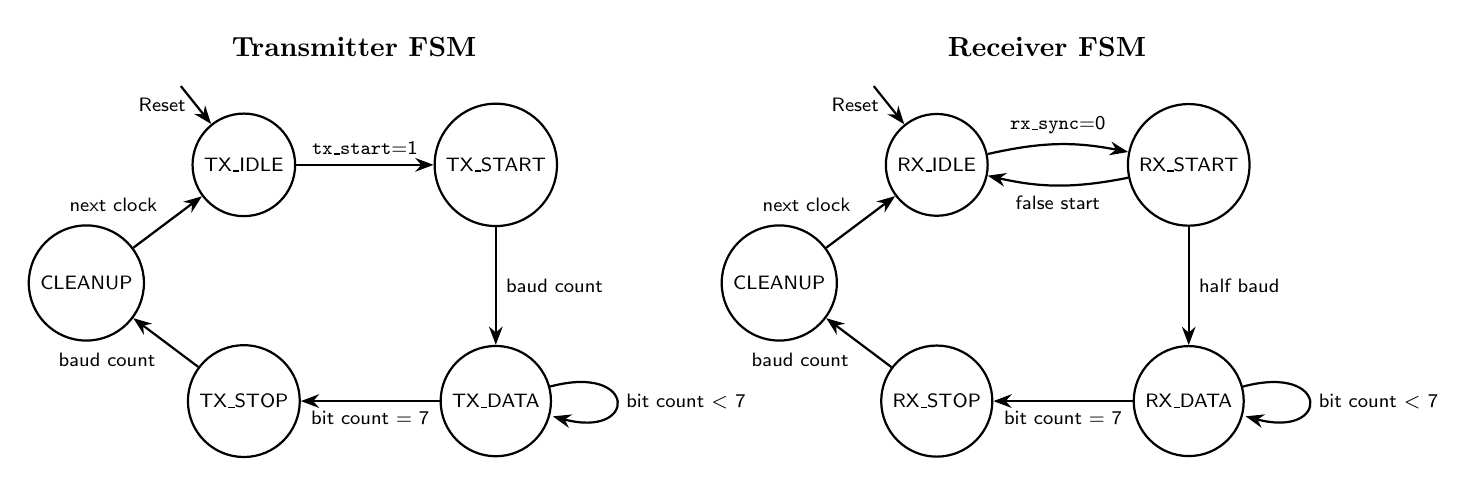
\begin{tikzpicture}[>=Stealth, thick, font=\sffamily\scriptsize,
state/.style={circle, draw, minimum size=1.25cm, align=center}]
    \node[state] (TX_IDLE) at (0, 0) {TX\_IDLE};
    \node[state] (TX_START) at (3.2, 0) {TX\_START};
    \node[state] (TX_DATA)  at (3.2, -3.0) {TX\_DATA};
    \node[state] (TX_STOP)  at (0, -3.0) {TX\_STOP};
    \node[state] (TX_CLEANUP) at (-2.0, -1.5) {CLEANUP};
    \draw[->] (-0.8,1.0) -- (TX_IDLE) node[midway,left] {Reset};
    \path[->]
        (TX_IDLE) edge node[above] {\texttt{tx\_start}=1} (TX_START)
        (TX_START) edge node[right] {baud count} (TX_DATA)
        (TX_DATA) edge[loop right] node {bit count $<$ 7} (TX_DATA)
                  edge node[below] {bit count = 7} (TX_STOP)
        (TX_STOP) edge node[below left] {baud count} (TX_CLEANUP)
        (TX_CLEANUP) edge node[above left] {next clock} (TX_IDLE);
    \node[above, font=\bfseries] at (1.4, 1.25) {Transmitter FSM};

    \begin{scope}[xshift=8.8cm]
        \node[state] (RX_IDLE) at (0, 0) {RX\_IDLE};
        \node[state] (RX_START) at (3.2, 0) {RX\_START};
        \node[state] (RX_DATA)  at (3.2, -3.0) {RX\_DATA};
        \node[state] (RX_STOP)  at (0, -3.0) {RX\_STOP};
        \node[state] (RX_CLEANUP) at (-2.0, -1.5) {CLEANUP};
        \draw[->] (-0.8,1.0) -- (RX_IDLE) node[midway,left] {Reset};
        \path[->]
            (RX_IDLE) edge[bend left=12] node[above] {\texttt{rx\_sync}=0} (RX_START)
            (RX_START) edge[bend left=12] node[below] {false start} (RX_IDLE)
                       edge node[right] {half baud} (RX_DATA)
            (RX_DATA) edge[loop right] node {bit count $<$ 7} (RX_DATA)
                      edge node[below] {bit count = 7} (RX_STOP)
            (RX_STOP) edge node[below left] {baud count} (RX_CLEANUP)
            (RX_CLEANUP) edge node[above left] {next clock} (RX_IDLE);
        \node[above, font=\bfseries] at (1.4, 1.25) {Receiver FSM};
    \end{scope}
\end{tikzpicture}}
\caption{Finite state machines for the UART transmitter (\texttt{tx.v}) and receiver (\texttt{rx.v}).}
\label{fig:uart_fsm}
\end{figure}

To integrate these operational sequences into the SoC, the UART peripheral is encapsulated within an APB wrapper module (\texttt{apb\_uart.v}), as depicted in Fig.~\ref{fig:uart_schem}. This hierarchical design isolates the raw serial logic (\texttt{uart\_core}) from the bus protocol logic, enhancing modularity.

\begin{figure}
\centering
\resizebox{0.9\textwidth}{!}{%
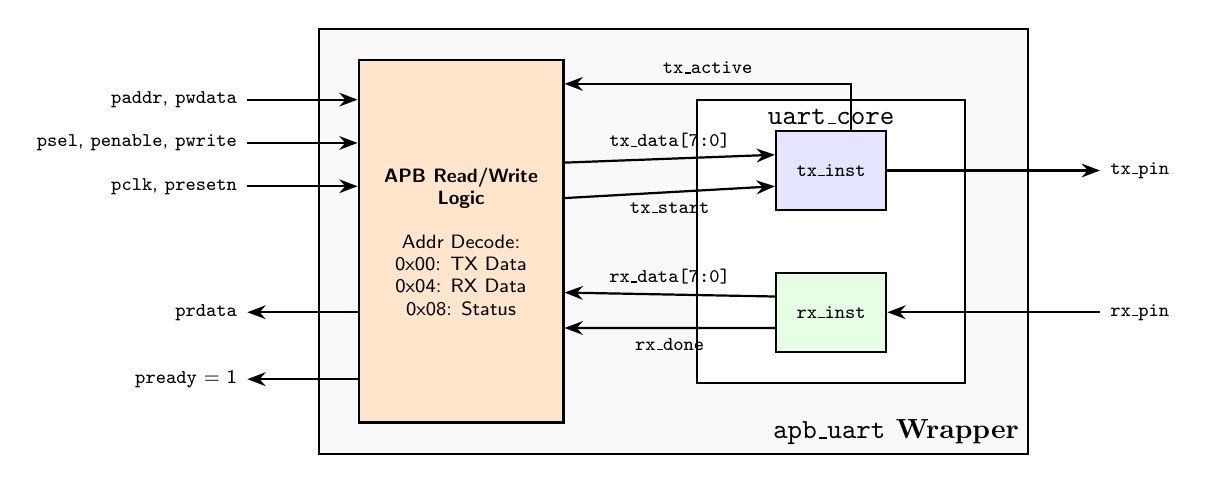
\begin{tikzpicture}[>=Stealth, thick, font=\sffamily\scriptsize]
    \node[draw, minimum width=9cm, minimum height=5.4cm, fill=gray!5] (apb_uart) at (0,0) {};
    \node[anchor=south east, font=\bfseries] at (apb_uart.south east) {\texttt{apb\_uart} Wrapper};
    \node[draw, minimum width=2.6cm, minimum height=4.6cm, align=center, fill=orange!20] (apb_if) at (-2.7,0) {\textbf{APB Read/Write}\\\textbf{Logic}\\\\Addr Decode:\\0x00: TX Data\\0x04: RX Data\\0x08: Status};
    \node[draw, minimum width=3.4cm, minimum height=3.6cm, fill=white] (uart_core) at (2,0) {};
    \node[anchor=north, font=\bfseries] at (uart_core.north) {\texttt{uart\_core}};
    \node[draw, minimum width=1.4cm, minimum height=1.0cm, fill=blue!10] (tx) at (2,0.9) {\texttt{tx\_inst}};
    \node[draw, minimum width=1.4cm, minimum height=1.0cm, fill=green!10] (rx) at (2,-0.9) {\texttt{rx\_inst}};
    \draw[<-] ([yshift=1.8cm]apb_if.west) -- ++(-1.4,0) node[anchor=east] {\texttt{paddr}, \texttt{pwdata}};
    \draw[<-] ([yshift=1.25cm]apb_if.west) -- ++(-1.4,0) node[anchor=east] {\texttt{psel}, \texttt{penable}, \texttt{pwrite}};
    \draw[<-] ([yshift=0.7cm]apb_if.west) -- ++(-1.4,0) node[anchor=east] {\texttt{pclk}, \texttt{presetn}};
    \draw[->] ([yshift=-0.9cm]apb_if.west) -- ++(-1.4,0) node[anchor=east] {\texttt{prdata}};
    \draw[->] ([yshift=-1.75cm]apb_if.west) -- ++(-1.4,0) node[anchor=east] {\texttt{pready} = 1};
    \draw[->] ([yshift=1.0cm]apb_if.east) -- ([yshift=0.2cm]tx.west) node[midway, above] {\texttt{tx\_data[7:0]}};
    \draw[->] ([yshift=0.55cm]apb_if.east) -- ([yshift=-0.2cm]tx.west) node[midway, below] {\texttt{tx\_start}};
    \draw[->] ([xshift=0.25cm]tx.north) |- ([yshift=2.0cm]apb_if.east) node[pos=0.75, above] {\texttt{tx\_active}};
    \draw[<-] ([yshift=-0.65cm]apb_if.east) -- ([yshift=0.2cm]rx.west) node[midway, above] {\texttt{rx\_data[7:0]}};
    \draw[<-] ([yshift=-1.1cm]apb_if.east) -- ([yshift=-0.2cm]rx.west) node[midway, below] {\texttt{rx\_done}};
    \draw[->] (tx.east) -- ++(2.7,0) node[anchor=west] {\texttt{tx\_pin}};
    \draw[<-] (rx.east) -- ++(2.7,0) node[anchor=west] {\texttt{rx\_pin}};
\end{tikzpicture}}
\caption{Detailed schematic of the UART module showing APB bus integration and internal block hierarchy.}
\label{fig:uart_schem}
\end{figure}

The APB wrapper provides three memory-mapped registers: transmit data at offset \texttt{0x00}, received data at offset \texttt{0x04}, and status at offset \texttt{0x08}. A transmit write generates \texttt{tx\_start}, while a receive read returns the stored byte and clears the receive-ready flag. Since the UART registers respond in one clock cycle, \texttt{pready} remains asserted and no APB wait states are required.

\subsection{Serial Peripheral Interface}

SPI is adopted in the proposed SoC as a synchronous full-duplex interface for high-speed peripheral communication \cite{mazidi2018,spiblockguide}. The interface uses four primary signals: SCLK, MOSI, MISO, and CS. The master generates the clock, selects the target device, shifts data through MOSI, and samples returned data through MISO, enabling simultaneous transmit and receive operation.

In the proposed architecture, the SPI controller is connected directly to the AHB-Lite interconnect rather than the APB domain. This placement provides lower-latency processor access for SPI transactions and is more suitable for data transfers that require deterministic timing. The SPI peripheral is exposed through memory-mapped transmit, receive, and status registers, allowing the processor to initiate transfers, poll completion, and retrieve received data through the AHB interface.

Figure~\ref{fig:spi_fsm} shows the FSM of the implemented SPI master core. The controller remains in \texttt{IDLE} with CS high and SCLK low until a transfer is started by the AHB wrapper. It then enters \texttt{TRANSFER}, drives CS low, shifts data on MOSI, and samples MISO while toggling SCLK. After all 8 bits are exchanged, the FSM passes through \texttt{WAIT\_CS} to stabilize the clock, then enters \texttt{DONE} to raise CS and generate a one-cycle completion pulse before returning to \texttt{IDLE}.

\begin{figure}
\centering
\resizebox{0.78\textwidth}{!}{%
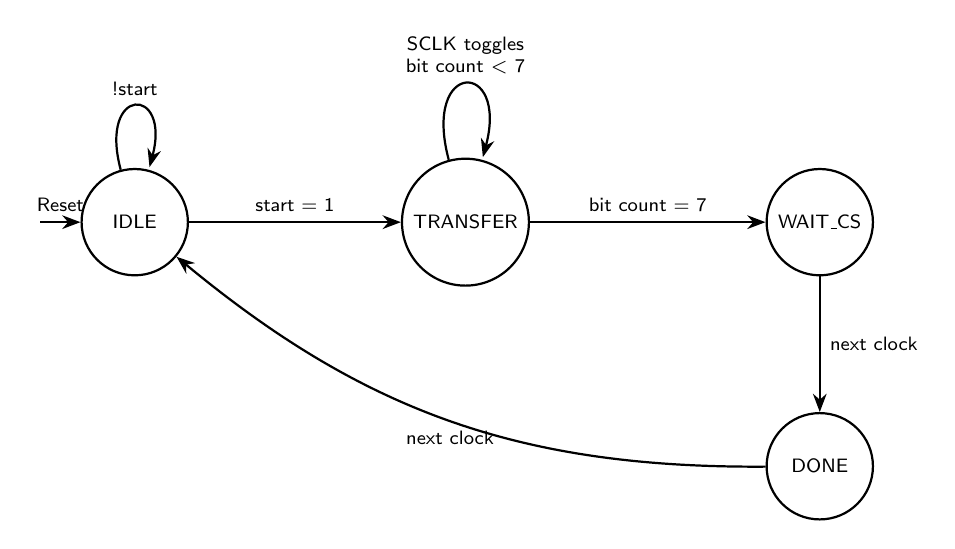
\begin{tikzpicture}[>=Stealth, node distance=2.7cm, on grid, auto, thick, font=\sffamily\scriptsize,
state/.style={circle, draw, minimum size=1.35cm, align=center}]
  \node[state] (IDLE) {IDLE};
  \node[state] (TRANSFER) [right=of IDLE, xshift=1.5cm] {TRANSFER};
  \node[state] (WAIT_CS) [right=of TRANSFER, xshift=1.8cm] {WAIT\_CS};
  \node[state] (DONE) [below=of WAIT_CS, yshift=-0.4cm] {DONE};
  \draw[->] (-1.2,0) -- (IDLE) node[midway, above] {Reset};
  \path[->]
    (IDLE) edge[loop above] node {!start} (IDLE)
           edge node {start = 1} (TRANSFER)
    (TRANSFER) edge[loop above] node[align=center] {SCLK toggles\\bit count $<$ 7} (TRANSFER)
               edge node {bit count = 7} (WAIT_CS)
    (WAIT_CS) edge node[right] {next clock} (DONE)
    (DONE) edge[bend left=20] node[below] {next clock} (IDLE);
\end{tikzpicture}}
\caption{Finite state machine for the SPI master controller (\texttt{spi\_master.v}).}
\label{fig:spi_fsm}
\end{figure}

To integrate this protocol into the SoC, the raw SPI master is encapsulated within an AHB-Lite wrapper (\texttt{ahb\_spi.v}), as shown in Fig.~\ref{fig:spi_schem}. To minimize logic gate overhead, this SPI peripheral omits configurable clock dividers and complex FIFO buffers, instead relying on instantaneous write logic and automated CS generation.

The SPI AHB wrapper exposes transmit, receive, and status registers at offsets \texttt{0x00}, \texttt{0x04}, and \texttt{0x08}. A processor write starts the SPI transfer, while the received byte is stored until it is read by software. The wrapper uses combinational read logic and keeps \texttt{hreadyout} asserted, allowing single-cycle AHB register access without bus stalling.

\begin{figure}
\centering
\resizebox{0.88\textwidth}{!}{%
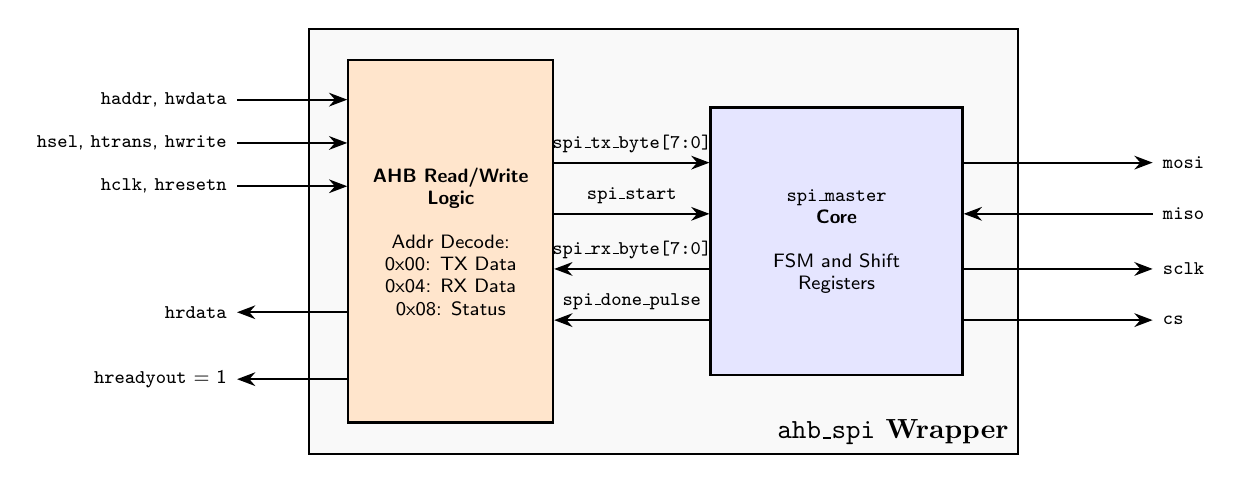
\begin{tikzpicture}[>=Stealth, thick, font=\sffamily\scriptsize]
    \node[draw, minimum width=9cm, minimum height=5.4cm, fill=gray!5] (ahb_spi) at (0,0) {};
    \node[anchor=south east, font=\bfseries] at (ahb_spi.south east) {\texttt{ahb\_spi} Wrapper};
    \node[draw, minimum width=2.6cm, minimum height=4.6cm, align=center, fill=orange!20] (ahb_if) at (-2.7,0) {\textbf{AHB Read/Write}\\\textbf{Logic}\\\\Addr Decode:\\0x00: TX Data\\0x04: RX Data\\0x08: Status};
    \node[draw, minimum width=3.2cm, minimum height=3.4cm, fill=blue!10, align=center] (spi_core) at (2.2,0) {\textbf{\texttt{spi\_master}}\\\textbf{Core}\\\\FSM and Shift\\Registers};
    \draw[<-] ([yshift=1.8cm]ahb_if.west) -- ++(-1.4,0) node[anchor=east] {\texttt{haddr}, \texttt{hwdata}};
    \draw[<-] ([yshift=1.25cm]ahb_if.west) -- ++(-1.4,0) node[anchor=east] {\texttt{hsel}, \texttt{htrans}, \texttt{hwrite}};
    \draw[<-] ([yshift=0.7cm]ahb_if.west) -- ++(-1.4,0) node[anchor=east] {\texttt{hclk}, \texttt{hresetn}};
    \draw[->] ([yshift=-0.9cm]ahb_if.west) -- ++(-1.4,0) node[anchor=east] {\texttt{hrdata}};
    \draw[->] ([yshift=-1.75cm]ahb_if.west) -- ++(-1.4,0) node[anchor=east] {\texttt{hreadyout} = 1};
    \draw[->] ([yshift=1.0cm]ahb_if.east) -- ([yshift=1.0cm]spi_core.west) node[midway, above] {\texttt{spi\_tx\_byte[7:0]}};
    \draw[->] ([yshift=0.35cm]ahb_if.east) -- ([yshift=0.35cm]spi_core.west) node[midway, above] {\texttt{spi\_start}};
    \draw[<-] ([yshift=-0.35cm]ahb_if.east) -- ([yshift=-0.35cm]spi_core.west) node[midway, above] {\texttt{spi\_rx\_byte[7:0]}};
    \draw[<-] ([yshift=-1.0cm]ahb_if.east) -- ([yshift=-1.0cm]spi_core.west) node[midway, above] {\texttt{spi\_done\_pulse}};
    \draw[->] ([yshift=1.0cm]spi_core.east) -- ++(2.4,0) node[anchor=west] {\texttt{mosi}};
    \draw[<-] ([yshift=0.35cm]spi_core.east) -- ++(2.4,0) node[anchor=west] {\texttt{miso}};
    \draw[->] ([yshift=-0.35cm]spi_core.east) -- ++(2.4,0) node[anchor=west] {\texttt{sclk}};
    \draw[->] ([yshift=-1.0cm]spi_core.east) -- ++(2.4,0) node[anchor=west] {\texttt{cs}};
\end{tikzpicture}}
\caption{Detailed schematic of the SPI controller showing the AHB-Lite bus wrapper and internal master core.}
\label{fig:spi_schem}
\end{figure}

\subsection{Inter-Integrated Circuit}

I\textsuperscript{2}C is adopted in the proposed SoC as a two-wire serial interface for low-speed peripheral communication \cite{i2cspec}. It uses SDA and SCL lines with open-drain behavior, allowing multiple devices to share the same bus while reducing pin usage compared with SPI.

A standard I\textsuperscript{2}C transaction begins with a START condition, followed by a 7-bit slave address, a read/write bit, an ACK response, data transfer, and a STOP condition. In the proposed SoC, this structure is used by the I\textsuperscript{2}C master to communicate with the internal slave model during verification. Although I\textsuperscript{2}C provides lower bandwidth than SPI, its compact two-wire structure makes it suitable for sensors, EEPROMs, and other low-speed SoC peripherals \cite{mazidi2018}.

The implemented I\textsuperscript{2}C master uses a quarter-period tick generator to control SDA and SCL timing. Each I\textsuperscript{2}C clock cycle is divided into four phases so that SDA is updated while SCL is low, sampled near the middle of the SCL-high period, and then advanced to the next bit.

As shown in Fig.~\ref{fig:i2c_fsm}, the FSM begins in \texttt{IDLE}, generates a \texttt{START} condition, sends the slave address, checks the ACK response, transfers data, and finally issues a \texttt{STOP} condition. If a NACK is detected after the address phase, the controller terminates the transaction and releases the bus.

\begin{figure}
\centering
\resizebox{0.95\textwidth}{!}{%
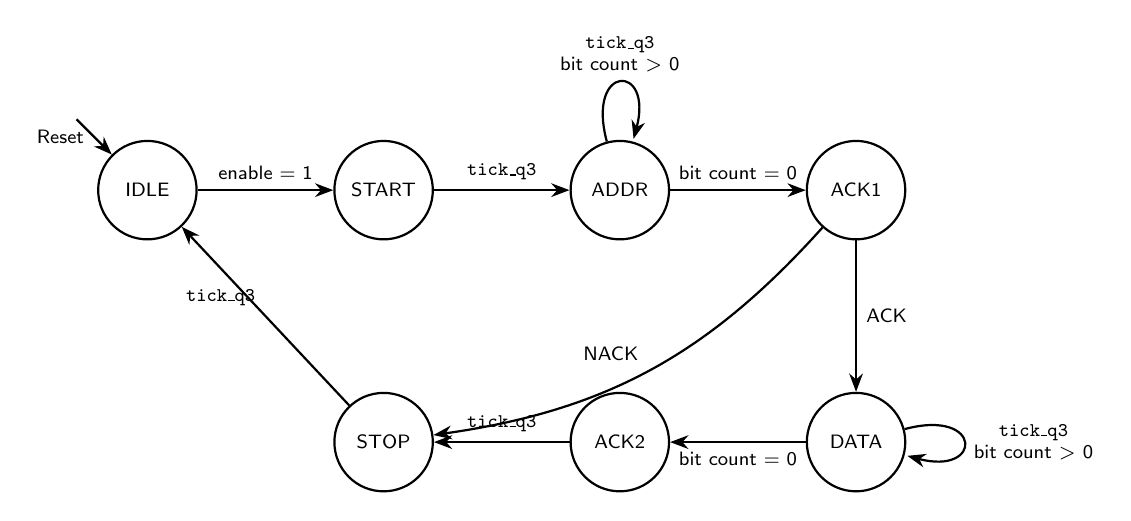
\begin{tikzpicture}[>=Stealth, on grid, auto, thick, font=\sffamily\scriptsize,
state/.style={circle, draw, minimum size=1.25cm, align=center}]
  \node[state] (IDLE) at (0,0) {IDLE};
  \node[state] (START) at (3,0) {START};
  \node[state] (ADDR) at (6,0) {ADDR};
  \node[state] (ACK1) at (9,0) {ACK1};
  \node[state] (DATA) at (9,-3.2) {DATA};
  \node[state] (ACK2) at (6,-3.2) {ACK2};
  \node[state] (STOP) at (3,-3.2) {STOP};
  \draw[->] (-0.9,0.9) -- (IDLE) node[midway,left] {Reset};
  \path[->]
    (IDLE) edge node[above] {enable = 1} (START)
    (START) edge node[above] {\texttt{tick\_q3}} (ADDR)
    (ADDR) edge[loop above] node[align=center] {\texttt{tick\_q3}\\bit count $>$ 0} (ADDR)
           edge node[above] {bit count = 0} (ACK1)
    (ACK1) edge node[right] {ACK} (DATA)
           edge[bend left=20] node[above left] {NACK} (STOP)
    (DATA) edge[loop right] node[align=center] {\texttt{tick\_q3}\\bit count $>$ 0} (DATA)
           edge node[below] {bit count = 0} (ACK2)
    (ACK2) edge node[above] {\texttt{tick\_q3}} (STOP)
    (STOP) edge node[above left] {\texttt{tick\_q3}} (IDLE);
\end{tikzpicture}}
\caption{Finite state machine for the I\textsuperscript{2}C master controller, driven by a quarter-period tick generator.}
\label{fig:i2c_fsm}
\end{figure}

The I\textsuperscript{2}C master is integrated into the SoC through an AHB-Lite wrapper, as shown in Fig.~\ref{fig:i2c_schem}. A write to offset \texttt{0x00} provides the slave address, read/write bit, and transmit data, while offset \texttt{0x08} reports busy status and offset \texttt{0x04} returns received data during read operations.

Because the I\textsuperscript{2}C core operates on a PMU-gated clock, the wrapper uses a two-flop synchronizer to transfer the enable signal from the always-on system clock domain into the gated I\textsuperscript{2}C clock domain. This prevents unreliable transaction start-up when the peripheral clock is re-enabled. The wrapper keeps \texttt{hreadyout} asserted, allowing the processor to access the peripheral without AHB wait states.

\begin{figure}
\centering
\resizebox{0.95\textwidth}{!}{%
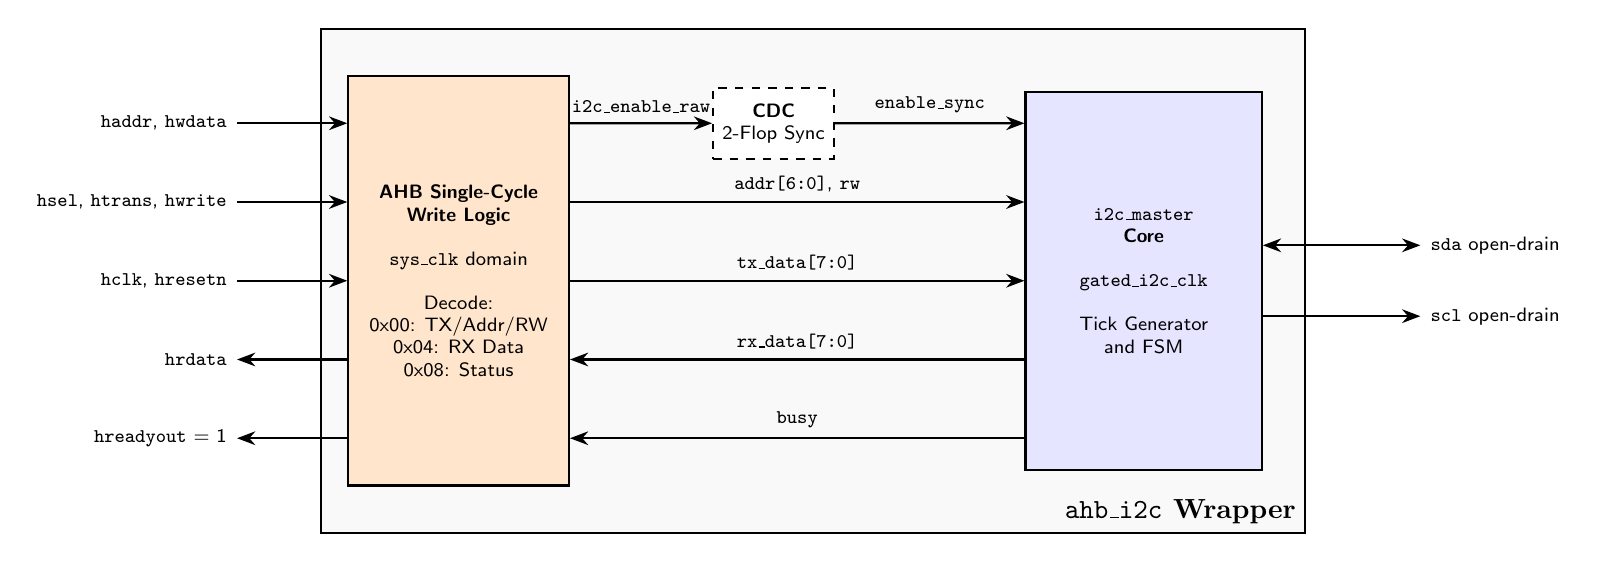
\begin{tikzpicture}[>=Stealth, thick, font=\sffamily\scriptsize]
    \node[draw, minimum width=12.5cm, minimum height=6.4cm, fill=gray!5] (ahb_i2c) at (0,0) {};
    \node[anchor=south east, font=\bfseries] at (ahb_i2c.south east) {\texttt{ahb\_i2c} Wrapper};
    \node[draw, minimum width=2.8cm, minimum height=5.2cm, align=center, fill=orange!20] (ahb_if) at (-4.5,0) {\textbf{AHB Single-Cycle}\\\textbf{Write Logic}\\\\\texttt{sys\_clk} domain\\\\Decode:\\0x00: TX/Addr/RW\\0x04: RX Data\\0x08: Status};
    \node[draw, dashed, minimum width=1.5cm, minimum height=0.9cm, fill=white, align=center] (cdc) at (-0.5,2.0) {\textbf{CDC}\\2-Flop Sync};
    \node[draw, minimum width=3.0cm, minimum height=4.8cm, fill=blue!10, align=center] (i2c_core) at (4.2,0) {\textbf{\texttt{i2c\_master}}\\\textbf{Core}\\\\\texttt{gated\_i2c\_clk}\\\\Tick Generator\\and FSM};
    \draw[<-] ([yshift=2.0cm]ahb_if.west) -- ++(-1.4,0) node[anchor=east] {\texttt{haddr}, \texttt{hwdata}};
    \draw[<-] ([yshift=1.0cm]ahb_if.west) -- ++(-1.4,0) node[anchor=east] {\texttt{hsel}, \texttt{htrans}, \texttt{hwrite}};
    \draw[<-] ([yshift=0cm]ahb_if.west) -- ++(-1.4,0) node[anchor=east] {\texttt{hclk}, \texttt{hresetn}};
    \draw[->] ([yshift=-1.0cm]ahb_if.west) -- ++(-1.4,0) node[anchor=east] {\texttt{hrdata}};
    \draw[->] ([yshift=-2.0cm]ahb_if.west) -- ++(-1.4,0) node[anchor=east] {\texttt{hreadyout} = 1};
    \draw[->] ([yshift=2.0cm]ahb_if.east) -- (cdc.west) node[midway, above] {\texttt{i2c\_enable\_raw}};
    \draw[->] (cdc.east) -- ([yshift=2.0cm]i2c_core.west) node[midway, above] {\texttt{enable\_sync}};
    \draw[->] ([yshift=1.0cm]ahb_if.east) -- ([yshift=1.0cm]i2c_core.west) node[midway, above] {\texttt{addr[6:0]}, \texttt{rw}};
    \draw[->] ([yshift=0.0cm]ahb_if.east) -- ([yshift=0.0cm]i2c_core.west) node[midway, above] {\texttt{tx\_data[7:0]}};
    \draw[<-] ([yshift=-1.0cm]ahb_if.east) -- ([yshift=-1.0cm]i2c_core.west) node[midway, above] {\texttt{rx\_data[7:0]}};
    \draw[<-] ([yshift=-2.0cm]ahb_if.east) -- ([yshift=-2.0cm]i2c_core.west) node[midway, above] {\texttt{busy}};
    \draw[<->] ([yshift=0.45cm]i2c_core.east) -- ++(2.0,0) node[anchor=west] {\texttt{sda} open-drain};
    \draw[->] ([yshift=-0.45cm]i2c_core.east) -- ++(2.0,0) node[anchor=west] {\texttt{scl} open-drain};
\end{tikzpicture}}
\caption{Detailed schematic of the I\textsuperscript{2}C controller illustrating the Clock Domain Crossing (CDC) synchronizer connecting the AHB interface to the gated I\textsuperscript{2}C master core.}
\label{fig:i2c_schem}
\end{figure}

\section{Experimental Results and Discussion}
\label{sec:results}

\subsection{Experimental Setup}

The proposed SoC communication subsystem was modeled at the register-transfer level (RTL) using Verilog hardware description language (HDL), following standard digital design and synthesis practices \cite{palnitkar2003,chu2008}. Functional simulation was performed using Xilinx Vivado XSim \cite{xilinx2018}. The system operates with a 100 MHz system clock and integrates a RISC-V processor core, AHB-Lite interconnect, AHB-to-APB bridge, PMU, Data RAM, UART, SPI, and I\textsuperscript{2}C controllers.

The verification program stored in instruction memory configures the PMU, enables the corresponding peripheral clock, initiates a communication transaction, polls the peripheral status register, and finally reads back the received data. Loopback-based verification was used to confirm correct transmit and receive behavior. For UART, the transmit pin was connected to the receive pin. For SPI, the MOSI signal was connected to MISO. For I\textsuperscript{2}C, an internal slave model was connected to the shared SDA and SCL lines through an open-drain bus with pull-up behavior.

This setup verifies not only the individual protocol controllers, but also the complete memory-mapped communication path from the processor, through the AMBA bus structure, into each peripheral wrapper, and finally to the physical protocol-level interface.

\subsection{Functional Verification}

Functional simulation was performed to validate the correctness of the integrated UART, SPI, and I\textsuperscript{2}C communication subsystems. The main objective was to confirm that each peripheral could be configured by the processor, execute a complete protocol transaction, and return the expected received data through its memory-mapped register interface.

Table~\ref{tab:loopback_results} summarizes the loopback verification results.

\begin{table}
\caption{Loopback verification results of the integrated communication peripherals}
\label{tab:loopback_results}
\centering
\begin{tabular}{lllll}
\hline
Peripheral & Verification Mode & TX Data & RX Data & Result\\
\hline
UART & TX-RX loopback & \texttt{0xAB} & \texttt{0xAB} & Pass\\
SPI & MOSI-MISO loopback & \texttt{0x5A} & \texttt{0x5A} & Pass\\
I\textsuperscript{2}C & Master read from slave & -- & \texttt{0xCD} & Pass\\
\hline
\end{tabular}
\end{table}

\subsection{System-Level Verification Overview}

Before evaluating each communication peripheral individually, a system-level verification was performed to confirm that the complete SoC operates as an integrated memory-mapped communication platform. The verification program is stored in instruction memory and executed by the RISC-V processor core after reset. During execution, the processor accesses the PMU, UART, SPI, and I\textsuperscript{2}C controllers through the AMBA-based interconnect.

The verification sequence consists of four main steps. First, the processor enables the required peripheral clock through the PMU. Second, it writes configuration or transmit data to the selected peripheral register. Third, it polls the peripheral status register until the transaction is complete. Finally, it reads back the received data and stores the result in data memory. This sequence verifies the complete data path from instruction execution, address decoding, bus transaction generation, peripheral control, protocol execution, and receive-data readback.

Figure~\ref{fig:wave_system} summarizes the system-level verification flow used in the simulation.

\begin{figure}
\centering
\includegraphics[width=0.95\textwidth]{photos/system_verification_waveform.png}
\caption{System-level verification flow showing CPU-controlled access to the PMU and communication peripherals through the AMBA interconnect.}
\label{fig:wave_system}
\end{figure}

The simulation results confirm that all three integrated communication peripherals complete their loopback or slave-response transactions successfully. The UART subsystem receives \texttt{0xAB}, the SPI subsystem receives \texttt{0x5A}, and the I\textsuperscript{2}C subsystem receives \texttt{0xCD}. These results demonstrate that the proposed SoC works correctly at both the system-interconnect level and the protocol-controller level.

\begin{table}
\caption{System-level verification sequence}
\label{tab:verification_sequence}
\centering
\begin{tabular}{lll}
\hline
Step & Operation & Purpose\\
\hline
1 & Enable peripheral clock through PMU & Validate clock-control path\\
2 & Write data/control register & Validate memory-mapped bus access\\
3 & Poll status register & Confirm transaction progress reporting\\
4 & Read receive register & Validate end-to-end data return path\\
5 & Store result to data memory & Confirm CPU-visible verification result\\
\hline
\end{tabular}
\end{table}

\subsubsection{UART Subsystem Verification.}
The UART subsystem was verified using an internal loopback connection in which the UART transmit output was connected directly to the receive input. Before transmission, the processor enabled the UART clock through the PMU and accessed the UART peripheral through the APB interface.

Figure~\ref{fig:wave_uart_start} shows the start of the UART transaction. The processor writes the test byte \texttt{0xAB} to the UART transmit register, which appears on \texttt{pwdata[31:0]} during an APB write access. After the write is accepted, the UART interface asserts \texttt{tx\_start}, loads \texttt{tx\_data\_in[7:0]} with \texttt{0xAB}, and raises \texttt{tx\_busy}. The serial frame then begins on \texttt{tx\_pin}, while the loopback connection drives the same signal onto \texttt{rx\_pin}.

\begin{figure}
\centering
\includegraphics[width=0.95\textwidth]{photos/uart_start_waveform.png}
\caption{UART APB write transaction initiating loopback transmission of \texttt{0xAB}.}
\label{fig:wave_uart_start}
\end{figure}

Figure~\ref{fig:wave_uart} shows the receive result after the complete UART frame has been transmitted through the loopback path. The receiver samples the looped-back serial signal and asserts \texttt{rx\_done} when the frame is complete. The received data register contains \texttt{0xAB}, matching the transmitted byte. This confirms correct UART transmission, reception, loopback behavior, status signaling, and APB register access.

\begin{figure}
\centering
\includegraphics[width=0.95\textwidth]{photos/uart_waveform.png}
\caption{UART loopback receive waveform showing successful recovery of \texttt{0xAB}.}
\label{fig:wave_uart}
\end{figure}

\subsubsection{SPI Subsystem Verification.}
The SPI subsystem was verified using a hardware loopback configuration where the MOSI signal was connected to the MISO input. The processor enabled the SPI clock through the PMU and wrote the test byte \texttt{0x5A} to the SPI transmit register. The AHB wrapper latched the transmit data and generated a \texttt{spi\_start} pulse to begin the transaction.

The SPI master asserted the chip-select signal, generated the serial clock, and shifted data out through MOSI while simultaneously sampling MISO. Because MOSI and MISO were connected in loopback, the received byte is expected to match the transmitted byte. The simulation result confirms that the SPI receive register captured \texttt{0x5A}, as shown in Fig.~\ref{fig:wave_spi}. The assertion of the \texttt{spi\_done} signal further confirms successful completion of the transaction.

\begin{figure}
\centering
\includegraphics[width=0.95\textwidth]{photos/spi_waveform.png}
\caption{SPI loopback simulation waveform showing MOSI-MISO transfer of \texttt{0x5A}.}
\label{fig:wave_spi}
\end{figure}

\subsubsection{I\textsuperscript{2}C Subsystem Verification.}
The I\textsuperscript{2}C subsystem was verified using an internal slave model connected to the shared SDA and SCL lines. The processor enabled the I\textsuperscript{2}C clock through the PMU and initiated a master-read transaction targeting slave address \texttt{0x57}. The slave model was configured to return the data byte \texttt{0xCD}.

As illustrated in Fig.~\ref{fig:wave_i2c}, the master first generates a START condition, followed by the 7-bit slave address and read bit. The slave acknowledges the address and then drives the data byte onto the SDA line. The master samples the incoming bits and stores the received value in the I\textsuperscript{2}C receive register. The simulation confirms that \texttt{i2c\_rx\_data} contains \texttt{0xCD}, matching the expected slave response.

This result verifies correct I\textsuperscript{2}C address transmission, read-mode operation, ACK handling, data reception, and STOP generation.

\begin{figure}
\centering
\includegraphics[width=0.95\textwidth]{photos/i2c_waveform.png}
\caption{I\textsuperscript{2}C master-read simulation waveform showing reception of \texttt{0xCD} from slave address \texttt{0x57}.}
\label{fig:wave_i2c}
\end{figure}

\subsection{Discussion}

The experimental results demonstrate that the proposed SoC communication subsystem operates correctly across both bus-level and protocol-level interfaces. The processor successfully configures each peripheral through memory-mapped registers, while the peripheral wrappers translate these bus transactions into protocol-specific control signals.

The loopback results provide direct evidence of correct end-to-end data movement. In the UART subsystem, the transmitted byte \texttt{0xAB} is recovered by the receiver, confirming correct serial framing and receive sampling. In the SPI subsystem, the byte \texttt{0x5A} is shifted through the MOSI-MISO loopback path, confirming correct full-duplex synchronous operation. In the I\textsuperscript{2}C subsystem, the master successfully reads \texttt{0xCD} from the slave at address \texttt{0x57}, confirming correct address decoding, ACK response, and read-data sampling.

A significant strength of the design is the separation between protocol logic and bus-interface logic, which follows modular SoC and reusable IP design principles \cite{wolf2012,furber2000,amba3ahb,amba3apb}. Each communication controller is implemented as an independent module and integrated through a lightweight AHB or APB wrapper. This makes the system easier to debug, verify, and extend. Additional peripherals can be added to the AHB-Lite interconnect or APB domain without major changes to the existing modules.

The results also show that PMU-based clock gating can be integrated into a communication subsystem without compromising functional correctness. By using protocol-specific grace periods, the design allows peripheral clocks to remain active until the ongoing transaction completes. This approach improves power-awareness while preserving reliable communication behavior.

Overall, the proposed architecture provides a compact and modular SoC communication subsystem suitable for embedded and IoT-oriented designs requiring multiple serial communication standards.

\section{Conclusion}
\label{sec:conclusion}

The implemented RISC-V-based SoC communication subsystem demonstrates correct integration of UART, SPI, and I\textsuperscript{2}C controllers within an AMBA memory-mapped architecture. The design connects SPI and I\textsuperscript{2}C directly to the AHB-Lite interconnect, while UART is accessed through an AHB-to-APB bridge. This organization matches the communication requirements of each peripheral and keeps the low-bandwidth UART interface separated from the main AHB-Lite peripheral path.

RTL simulation verified the complete processor-controlled communication flow, including PMU clock enabling, memory-mapped register access, protocol execution, status polling, receive-data readback, and result storage. The UART loopback test successfully recovered \texttt{0xAB}, confirming correct transmit framing, receive sampling, and APB register behavior. The SPI loopback test recovered \texttt{0x5A}, confirming correct MOSI-MISO transfer and completion signaling. The I\textsuperscript{2}C master-read test received \texttt{0xCD} from slave address \texttt{0x57}, confirming correct address transmission, ACK handling, and read-data capture.

The verification results show that the peripheral wrappers and protocol controllers operate correctly together as a single communication subsystem. The PMU clock-gating mechanism also functions with protocol-specific grace periods, allowing ongoing transactions to complete before peripheral clocks are disabled. This preserves functional correctness while still allowing unused peripherals to be disabled during idle periods.

The main finding is that a compact bus-based organization can support multiple serial protocols while keeping protocol logic and bus-interface logic separated. Each controller remains independently structured, while the wrapper modules provide the memory-mapped interface required by the processor. This separation simplifies verification and supports future extension of the communication subsystem.

Future work will focus on FPGA deployment, interrupt-driven control, configurable timing registers, FIFO buffering, and direct memory access (DMA) support. These extensions would improve hardware validation, processor efficiency, timing flexibility, and data-transfer throughput while preserving the modular bus-based structure of the current design.

\begin{thebibliography}{14}

\bibitem{wolf2012}
Wolf, W.: Computers as Components: Principles of Embedded Computing System Design, 3rd edn. Morgan Kaufmann, Waltham, MA (2012)

\bibitem{furber2000}
Furber, S.: ARM System-on-Chip Architecture, 2nd edn. Addison-Wesley, Boston, MA (2000)

\bibitem{patterson2021}
Patterson, D.A., Hennessy, J.L.: Computer Organization and Design RISC-V Edition: The Hardware Software Interface, 2nd edn. Morgan Kaufmann, Cambridge, MA (2021)

\bibitem{mazidi2018}
Mazidi, M.A., Mazidi, J.G., McKinlay, R.D.: The 8051 Microcontroller and Embedded Systems: Using Assembly and C, 2nd edn. Pearson, Upper Saddle River, NJ (2018)

\bibitem{serialportcomplete}
Axelson, J.: Serial Port Complete: COM Ports, USB Virtual COM Ports, and Ports for Embedded Systems, 2nd edn. Lakeview Research, Madison, WI (2007)

\bibitem{spiblockguide}
Freescale Semiconductor: SPI Block Guide, 3.06 edn. Freescale Semiconductor (2003)

\bibitem{i2cspec}
NXP Semiconductors: UM10204 I2C-bus Specification and User Manual, 7th edn. NXP Semiconductors (2021)

\bibitem{amba3ahb}
Arm Limited: AMBA 3 AHB-Lite Protocol Specification. Arm Limited (2006). ARM IHI 0033A

\bibitem{amba3apb}
Arm Limited: AMBA 3 APB Protocol Specification. Arm Limited (2006). ARM IHI 0024B

\bibitem{riscv2019}
RISC-V Foundation: The RISC-V Instruction Set Manual, Volume I: Unprivileged ISA. RISC-V Foundation (2019). Document Version 20191213

\bibitem{rabaey2003}
Rabaey, J.M., Chandrakasan, A., Nikolic, B.: Digital Integrated Circuits: A Design Perspective, 2nd edn. Prentice Hall, Upper Saddle River, NJ (2003)

\bibitem{palnitkar2003}
Palnitkar, S.: Verilog HDL: A Guide to Digital Design and Synthesis, 2nd edn. Prentice Hall, Upper Saddle River, NJ (2003)

\bibitem{chu2008}
Chu, P.P.: FPGA Prototyping by Verilog Examples: Xilinx Spartan-3 Version. Wiley, Hoboken, NJ (2008)

\bibitem{xilinx2018}
Xilinx: Vivado Design Suite User Guide: Logic Simulation. Xilinx (2018). UG900

\end{thebibliography}

\end{document}
